\documentclass[11pt,a4paper]{article}
\usepackage[utf8]{inputenc}
\usepackage[margin=1in]{geometry}
\usepackage{graphicx}
\usepackage[hidelinks]{hyperref}
\usepackage{xcolor}
\usepackage{fancyhdr}
\usepackage{titlesec}
\usepackage{enumitem}
\usepackage{tcolorbox}
\usepackage{fontawesome5}

% Colors
\definecolor{primarygreen}{RGB}{46,125,50}
\definecolor{accentgreen}{RGB}{76,175,80}
\definecolor{lightgray}{RGB}{248,249,250}

% Header and footer
\setlength{\headheight}{15pt}
\addtolength{\topmargin}{-3pt}
\pagestyle{fancy}
\fancyhf{}
\fancyhead[L]{\textcolor{primarygreen}{\textbf{PLS 120 - Week 1 Tutorial}}}
\fancyhead[R]{\textcolor{primarygreen}{UC Davis}}
\fancyfoot[C]{\thepage}

% Title formatting
\titleformat{\section}{\Large\bfseries\color{primarygreen}}{}{0em}{}[\titlerule]
\titleformat{\subsection}{\large\bfseries\color{primarygreen}}{}{0em}{}

% Custom boxes
\newtcolorbox{infobox}{
    colback=lightgray,
    colframe=primarygreen,
    boxrule=1pt,
    arc=3pt,
    left=10pt,
    right=10pt,
    top=10pt,
    bottom=10pt
}

\newtcolorbox{warningbox}{
    colback=accentgreen!10,
    colframe=primarygreen,
    boxrule=1pt,
    arc=3pt,
    left=10pt,
    right=10pt,
    top=10pt,
    bottom=10pt
}

\begin{document}

% Title page
\begin{titlepage}
    \centering
    \vspace*{2cm}
    
    {\Huge\bfseries\color{primarygreen} PLS 120: Applied Statistics in Agricultural Sciences}
    
    \vspace{1cm}
    
    {\Large\color{primarygreen} Interactive R Programming with Binder}
    
    \vspace{2cm}
    
    
\includegraphics[width=0.3\textwidth]{../../images/logos/Home_Page_Logo.png}
    
    \vspace{2cm}
    
    {\large\bfseries Week 1 Tutorial Guide}
    
    \vspace{1cm}
    
    {\large Mohammadreza Narimani}\\
    {\normalsize Department of Biological and Agricultural Engineering}\\
    {\normalsize University of California, Davis}
    
    \vspace{1cm}
    
    {\normalsize mnarimani@ucdavis.edu}
    
    \vfill
    
    {\normalsize October 2025}
\end{titlepage}

\tableofcontents
\newpage

\section{Important Links}

\begin{tcolorbox}[colback=accentgreen!20, colframe=primarygreen, boxrule=2pt, arc=5pt, title={\textbf{\Large Essential Course Resources}}]
\centering
\textbf{\Large Course Website}\\[0.5cm]
\textcolor{primarygreen}{\textbf{All course materials are available at:}}\\[0.3cm]
\href{https://mohammadrezanarimaniucdavis.github.io/PLS120-Statistics-Lab-Materials/}{\textbf{\Large \textcolor{primarygreen}{\underline{Click Here to Access Course Website}}}}\\[0.8cm]

\textbf{\Large Interactive Binder Environment}\\[0.5cm]
\textcolor{primarygreen}{\textbf{Access Week 1 lab materials directly:}}\\[0.3cm]
\href{https://mybinder.org/v2/gh/MohammadrezaNarimaniUCDavis/PLS120-Statistics-Lab-Materials/binder-week1}{\textbf{\Large \textcolor{primarygreen}{\underline{Click Here to Launch Binder}}}}
\end{tcolorbox}

\section{Welcome to PLS 120!}

In this course, we use the \textbf{R programming language} for statistical analysis in agriculture. Instead of installing R and RStudio on your computer, we use \textbf{Binder} and \textbf{Jupyter Notebooks} to provide you with a ready-to-use environment. No software installation needed!

\section{Why Use Binder?}

\begin{infobox}
\textbf{Benefits of Using Binder:}
\begin{itemize}[leftmargin=*]
    \item \textbf{No Installation Required} - Everything runs in your browser
    \item \textbf{Pre-configured Environment} - All packages already installed
    \item \textbf{Cross-platform} - Works on Windows, Mac, Linux
    \item \textbf{Always Updated} - Latest versions of R and packages
    \item \textbf{Easy Sharing} - Just click a link to get started
\end{itemize}
\end{infobox}

\section{Getting Started: Step-by-Step Guide}

\subsection{Step 1: Launch Binder Environment}

Click the \textbf{"Launch Binder"} button to start your R environment. This will take \textbf{2-5 minutes} to load.

\begin{center}
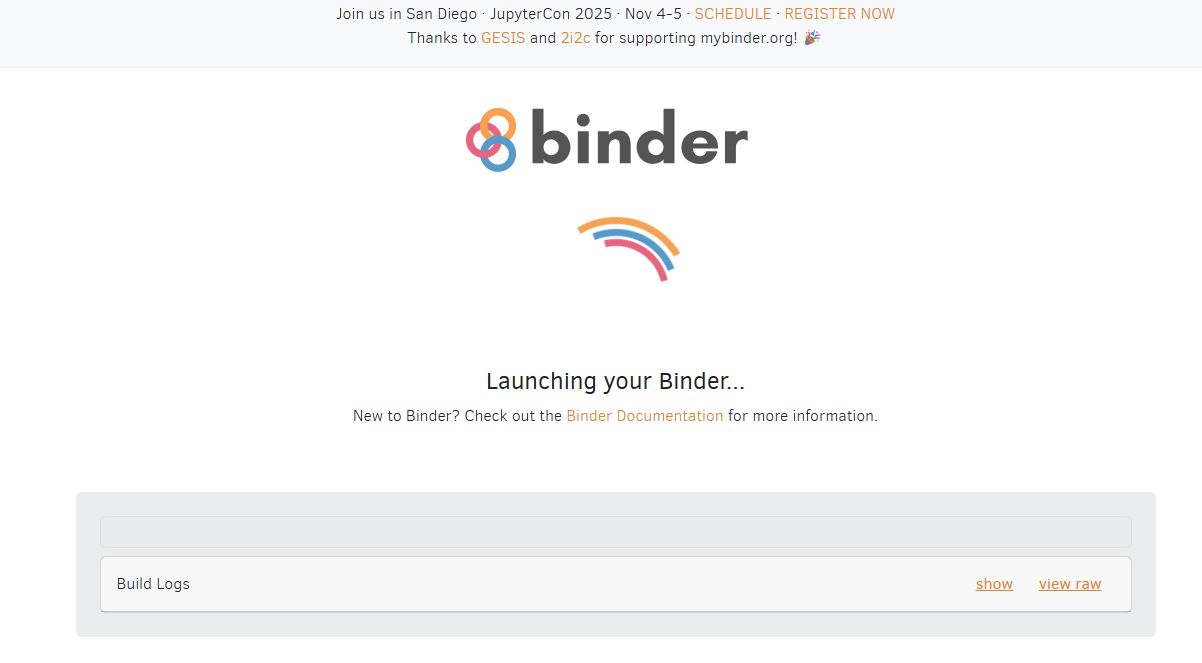
\includegraphics[width=0.8\textwidth]{../Image_1.png}\\
\textit{Binder is launching your environment - please wait patiently!}
\end{center}

\subsection{Step 2: Wait for Environment to Load}

After clicking the link, Binder will show progress through several stages:
\begin{itemize}
    \item \textbf{Waiting}
    \item \textbf{Building}
    \item \textbf{Pushing}
    \item \textbf{Launching}
\end{itemize}

The green progress bar shows Binder is almost ready!

\begin{center}
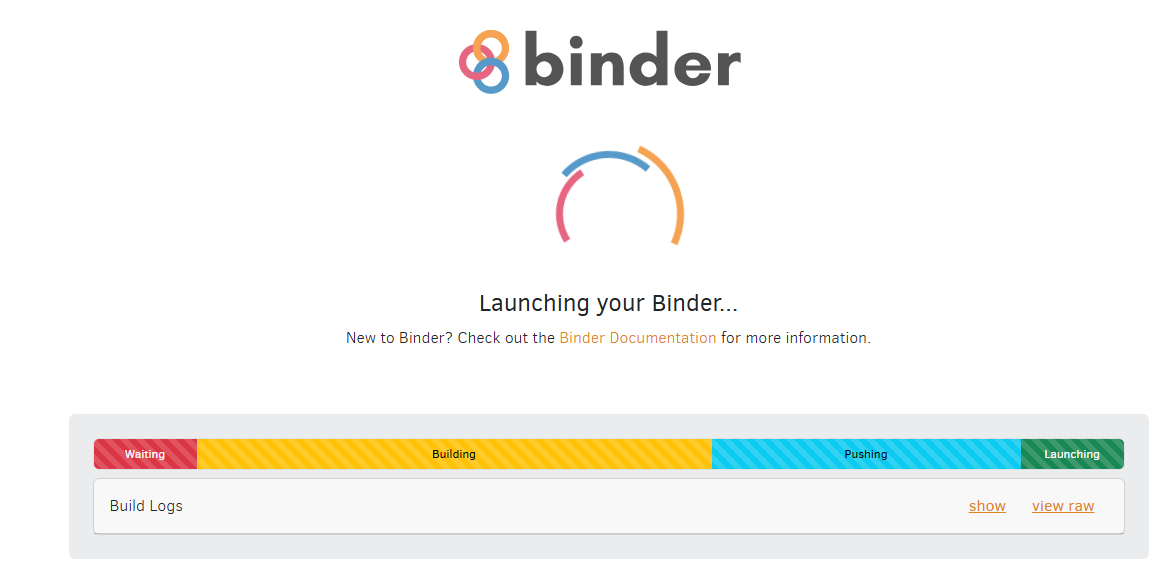
\includegraphics[width=0.8\textwidth]{../Image_2.png}\\
\textit{Green bar means your environment is ready in just a few seconds!}
\end{center}

\subsection{Step 3: Navigate to Class Activity}

Once Binder loads, you'll see the Jupyter Notebook interface. In the \textbf{left panel}, you'll see several folders:
\begin{itemize}
    \item \texttt{assignment/} - Your homework assignments
    \item \texttt{class\_activity/} - Lab tutorials and exercises
    \item Various files (README.md, runtime.txt, etc.)
\end{itemize}

\textbf{Click on the \texttt{class\_activity} folder} to access this week's content.

\begin{center}
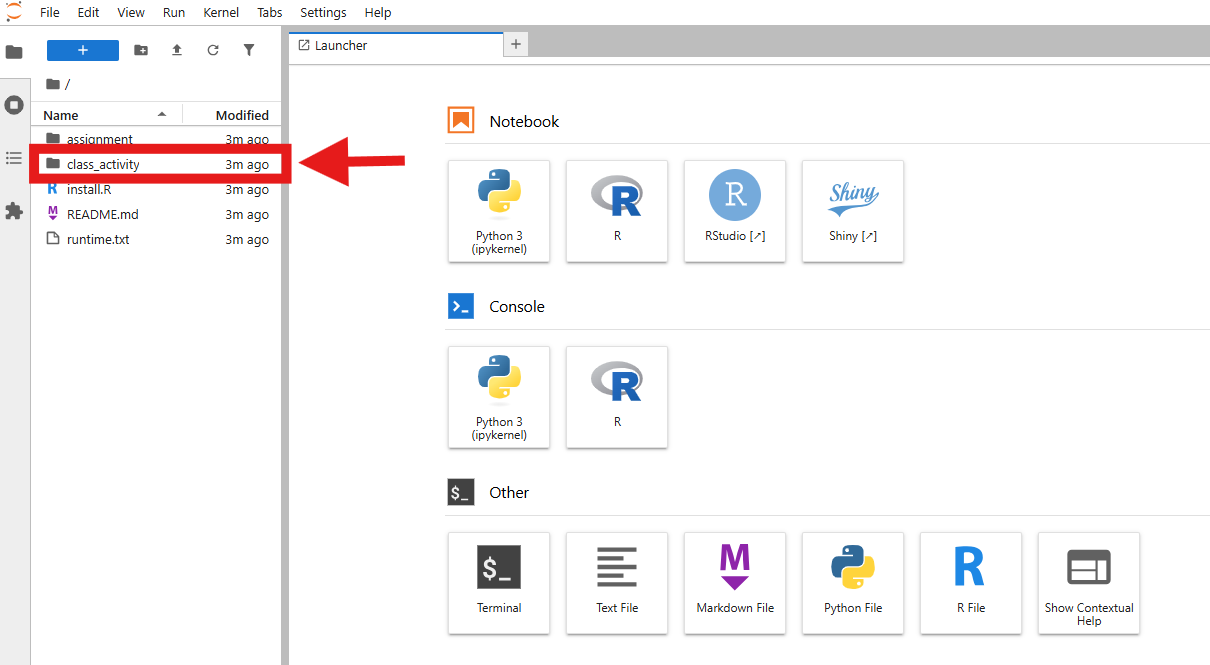
\includegraphics[width=0.8\textwidth]{../Image_3.png}\\
\textit{Click here to access your lab materials}
\end{center}

\subsection{Step 4: Open the Lab Notebook}

Inside the \texttt{class\_activity} folder, \textbf{double-click} on \texttt{Week1\_Introduction.ipynb} to open the interactive lab notebook.

\begin{center}
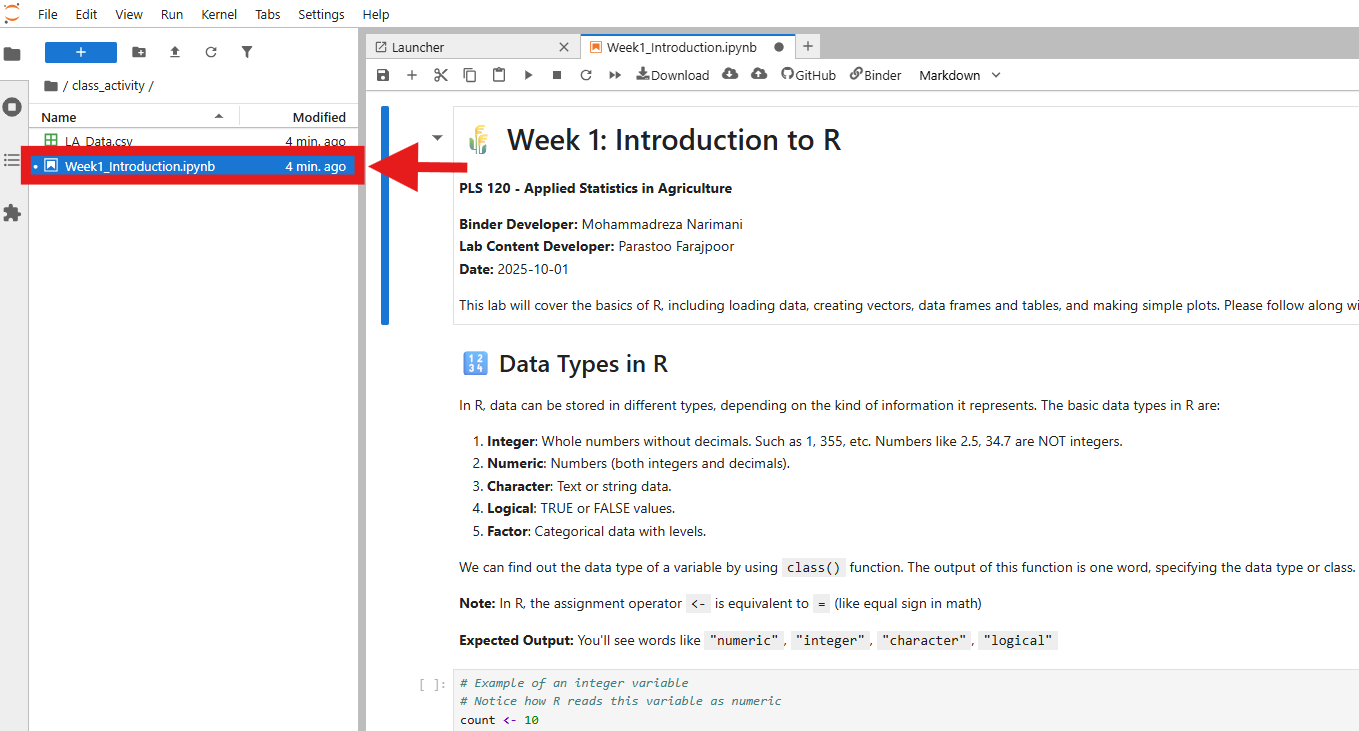
\includegraphics[width=0.8\textwidth]{../Image_4.png}\\
\textit{Double-click here to open the lab instructions and code}
\end{center}

\subsection{Step 5: Explore the Data (Optional)}

We've already uploaded the data for this lab! The file \texttt{LA\_Data.csv} contains the crime statistics data. You can \textbf{double-click} on it to explore the data if you're curious.

\begin{center}
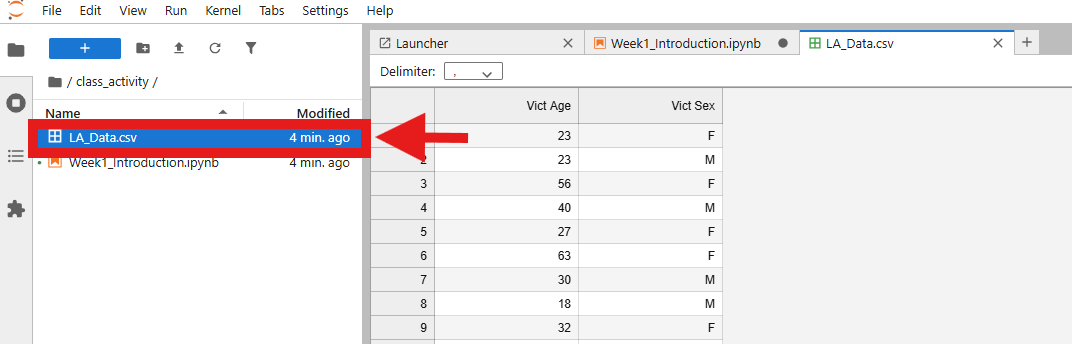
\includegraphics[width=0.8\textwidth]{../Image_5.png}\\
\textit{Click here to view the raw data (optional)}
\end{center}

\section{Saving Your Work}

\begin{warningbox}
\textbf{Important:} Binder environments are temporary! Always save your work locally.
\end{warningbox}

\subsection{Download Your Notebook}

When you're done working, save your progress:

\begin{enumerate}
    \item \textbf{Go back to main folder} - Click the folder icon in the left panel
\end{enumerate}

\begin{center}
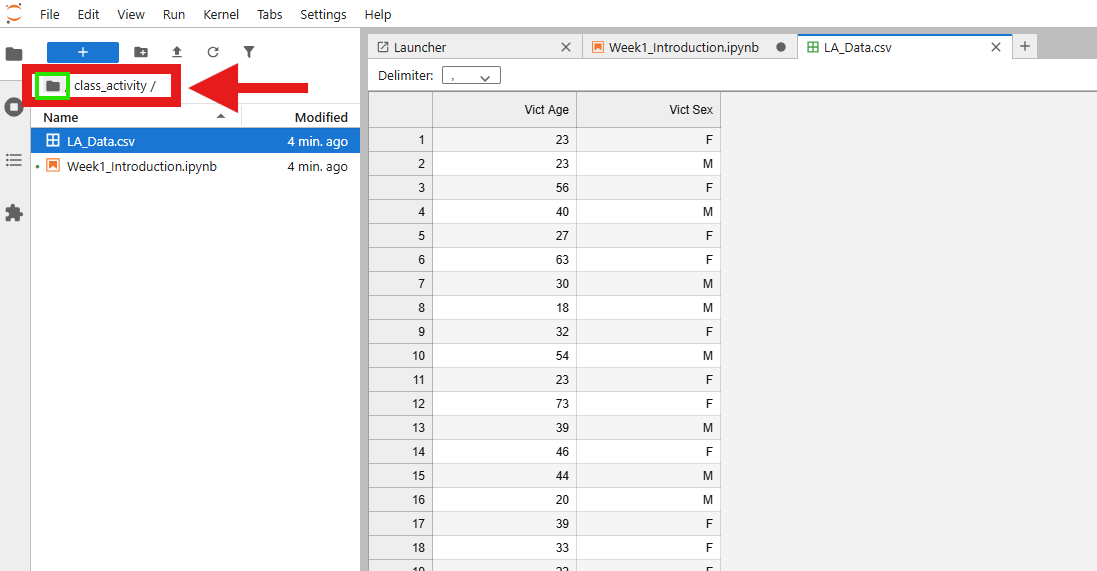
\includegraphics[width=0.8\textwidth]{../Image_6.png}\\
\textit{Click the folder icon to return to the main directory}
\end{center}

\begin{enumerate}[resume]
    \item \textbf{Download your notebook} - Right-click on your \texttt{.ipynb} file and select "Download"
\end{enumerate}

\section{Completing Assignments}

\subsection{Step 1: Access Assignment Folder}

From the main directory, \textbf{click on the \texttt{assignment} folder} to access your homework.

\begin{center}
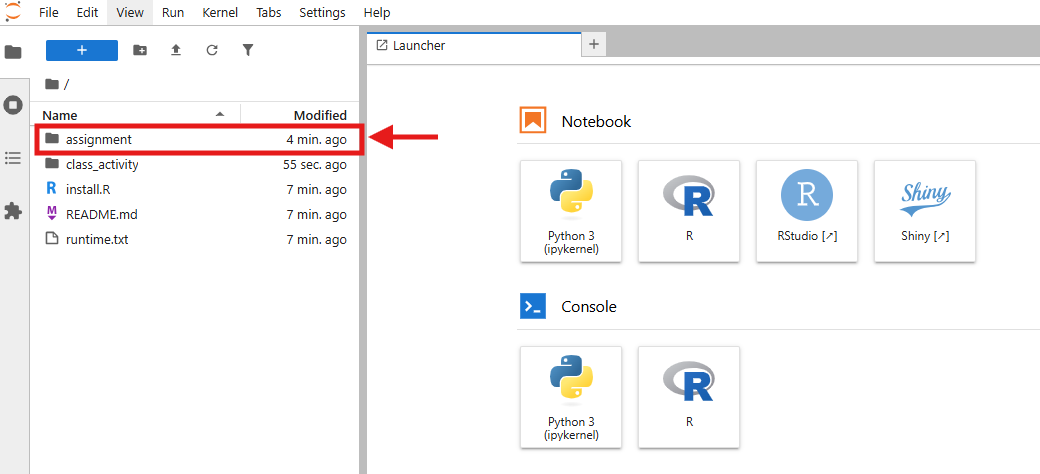
\includegraphics[width=0.8\textwidth]{../Image_7.png}\\
\textit{Click here to access assignment materials}
\end{center}

\subsection{Step 2: Open Assignment Notebook}

\textbf{Double-click} on \texttt{Assignment1.ipynb} to open your assignment.

\begin{center}
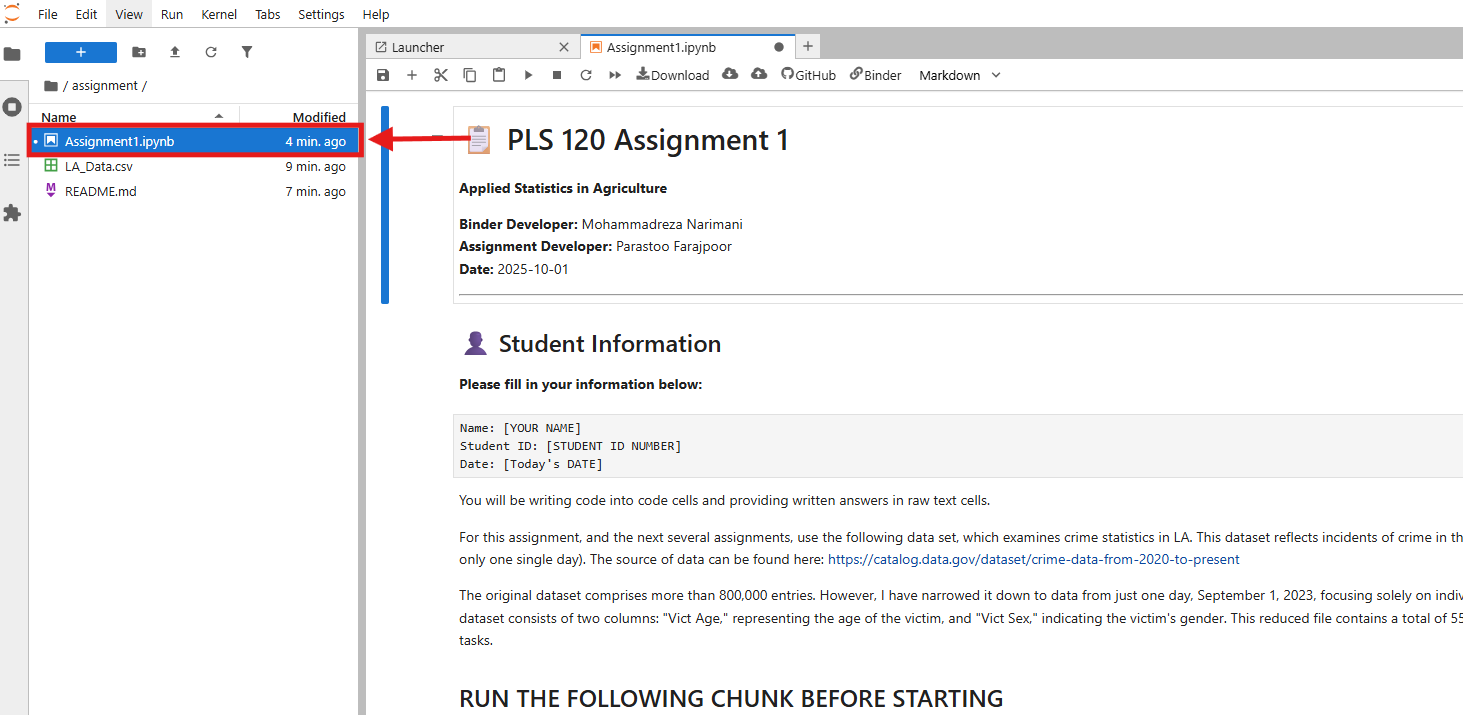
\includegraphics[width=0.8\textwidth]{../Image_8.png}\\
\textit{Double-click here to open your assignment}
\end{center}

\subsection{Step 3: Complete Your Work}

Fill in all \textbf{code boxes} and \textbf{text boxes} carefully to answer all questions. Look for:
\begin{itemize}
    \item Question mark emojis indicating questions to answer
    \item Code cells with hints in comments
    \item Raw text cells for your written responses
\end{itemize}

\subsection{Step 4: Download Your Completed Work}

\subsubsection{Download Code File (.ipynb)}

Click \textbf{File} → \textbf{Download} to save your notebook code.

\begin{center}
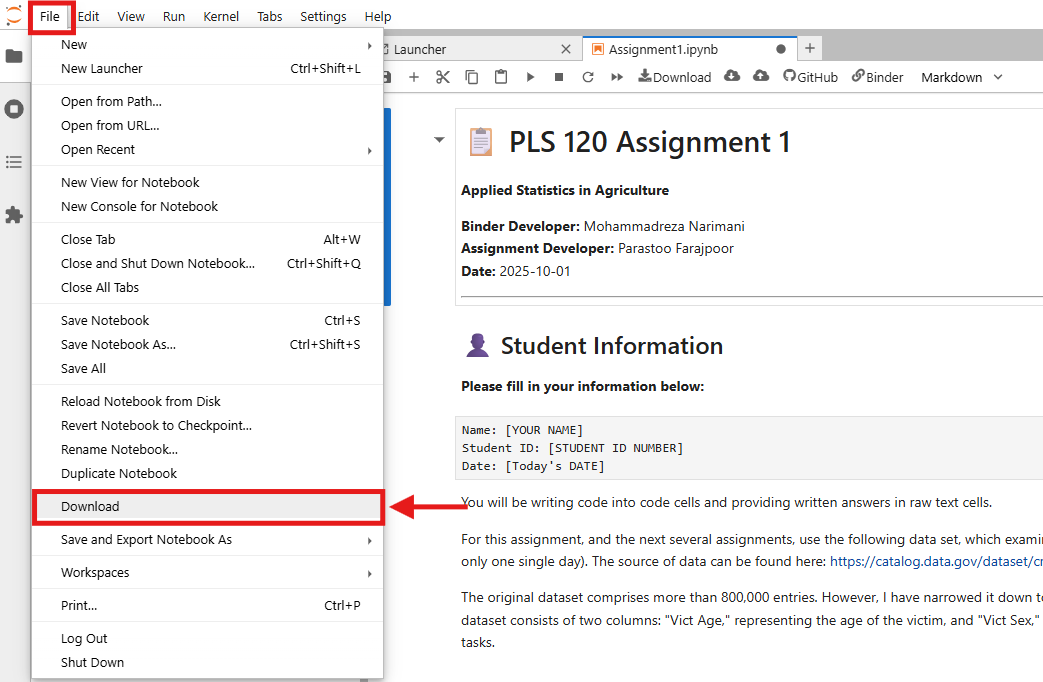
\includegraphics[width=0.8\textwidth]{../Image_9.png}\\
\textit{Download your .ipynb file for backup}
\end{center}

\subsubsection{Export HTML/PDF Report}

For submission, you also need an HTML or PDF report:

Click \textbf{File} → \textbf{Save and Export Notebook As} → \textbf{HTML} (or PDF)

\begin{center}
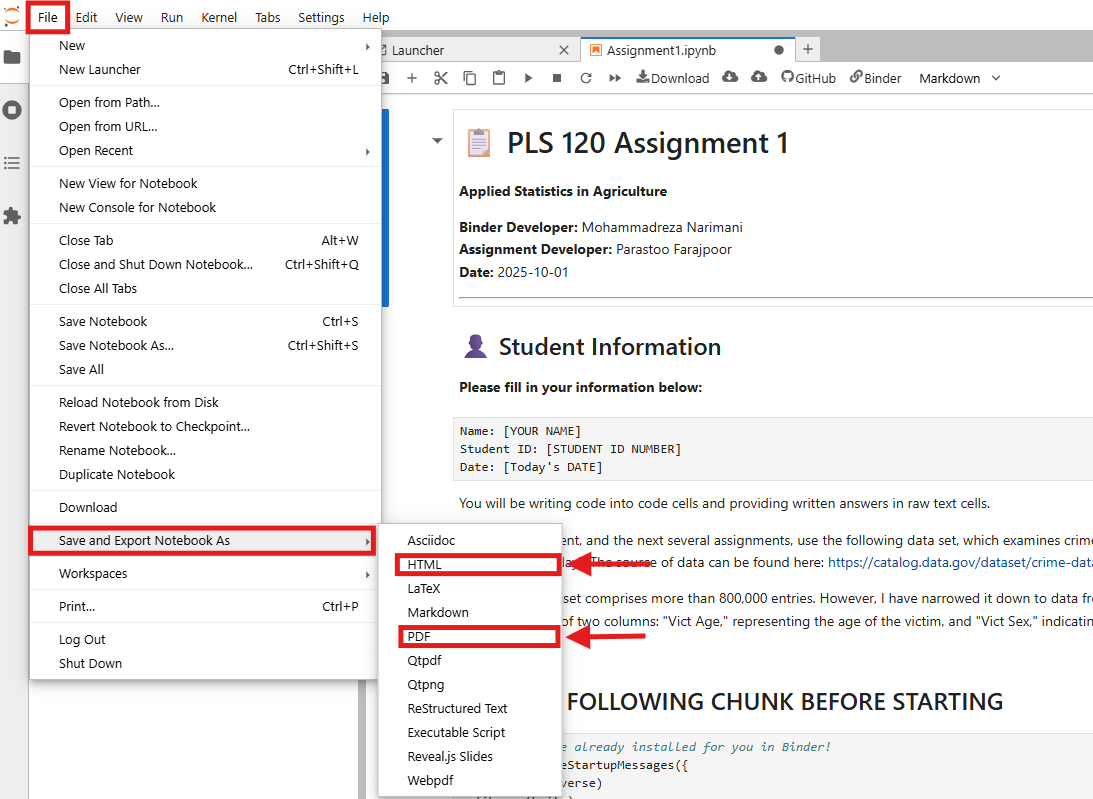
\includegraphics[width=0.8\textwidth]{../Image_10.png}\\
\textit{Export your completed assignment as HTML or PDF}
\end{center}

\section{Submission Requirements}

For each assignment, submit \textbf{TWO files} to UC Davis Canvas:

\begin{enumerate}
    \item \textbf{HTML/PDF Report} - Your formatted assignment with outputs
    \item \textbf{.ipynb File} - Your notebook code as backup
\end{enumerate}

\section{Important: Saving Your Progress}

\begin{warningbox}
\textbf{Do not close Binder if you have not saved your code or all your progress will be gone!}
\end{warningbox}

If you want to take a break and continue your activity or assignment later:

\subsection{Save Your Work Before Closing}

Right-click on your code (\texttt{.ipynb}) file and click "Download" to make sure you have saved your code locally.

\begin{center}
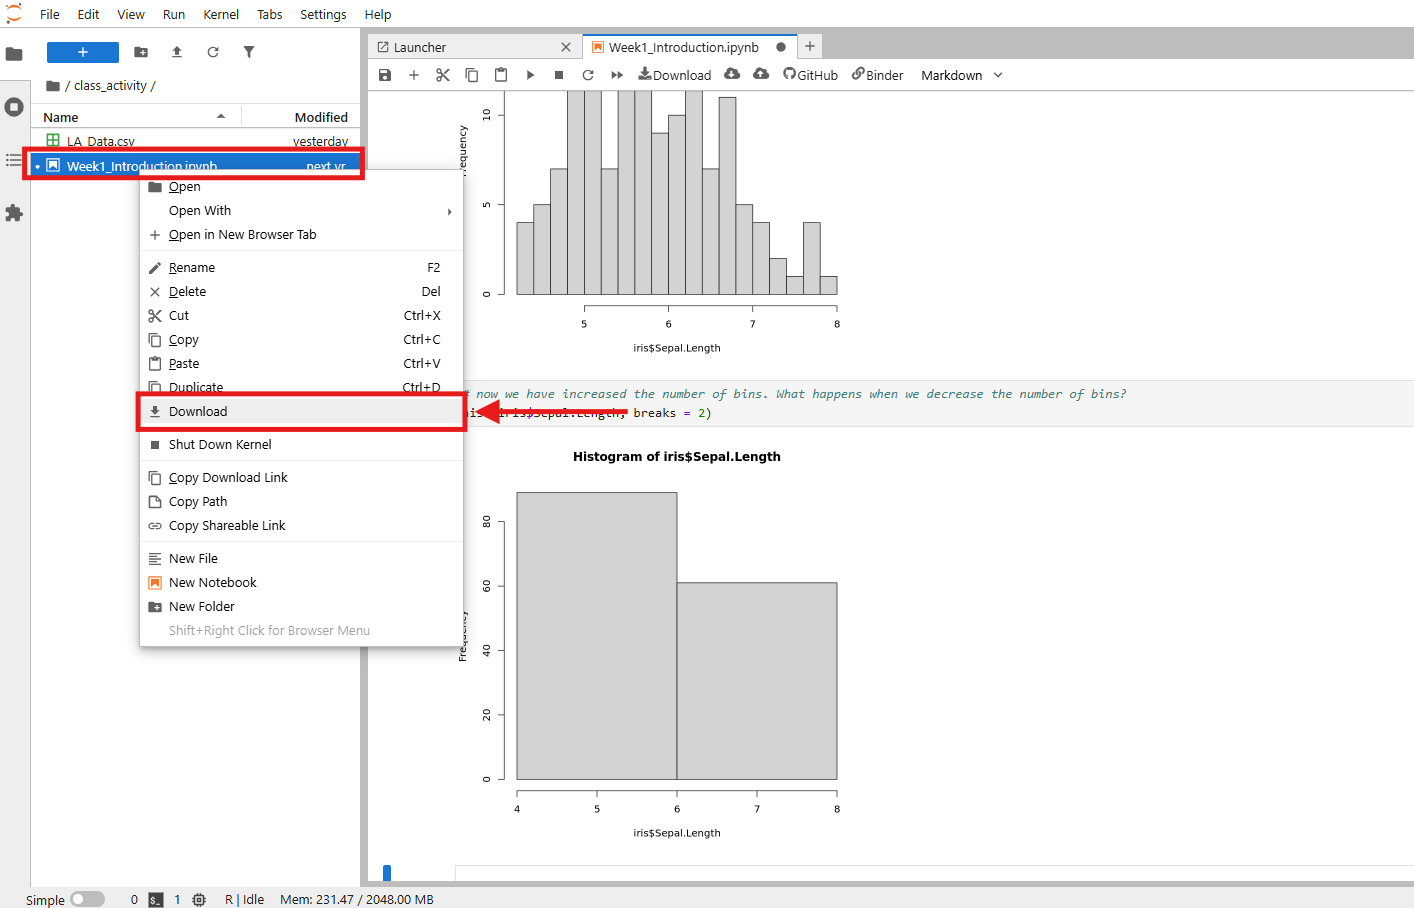
\includegraphics[width=0.8\textwidth]{../Image_11.png}\\
\textit{Right-click on your notebook file and download it before closing Binder}
\end{center}

\subsection{Continue Your Progress Later}

When you open Binder again and want to continue your work:

\begin{enumerate}
    \item Click the \textbf{Upload} button on the top ribbon
    \item Find your saved code file locally on your computer
    \item Upload your \texttt{.ipynb} file
    \item Run your code cells again to see your previous outputs!
\end{enumerate}

\begin{center}
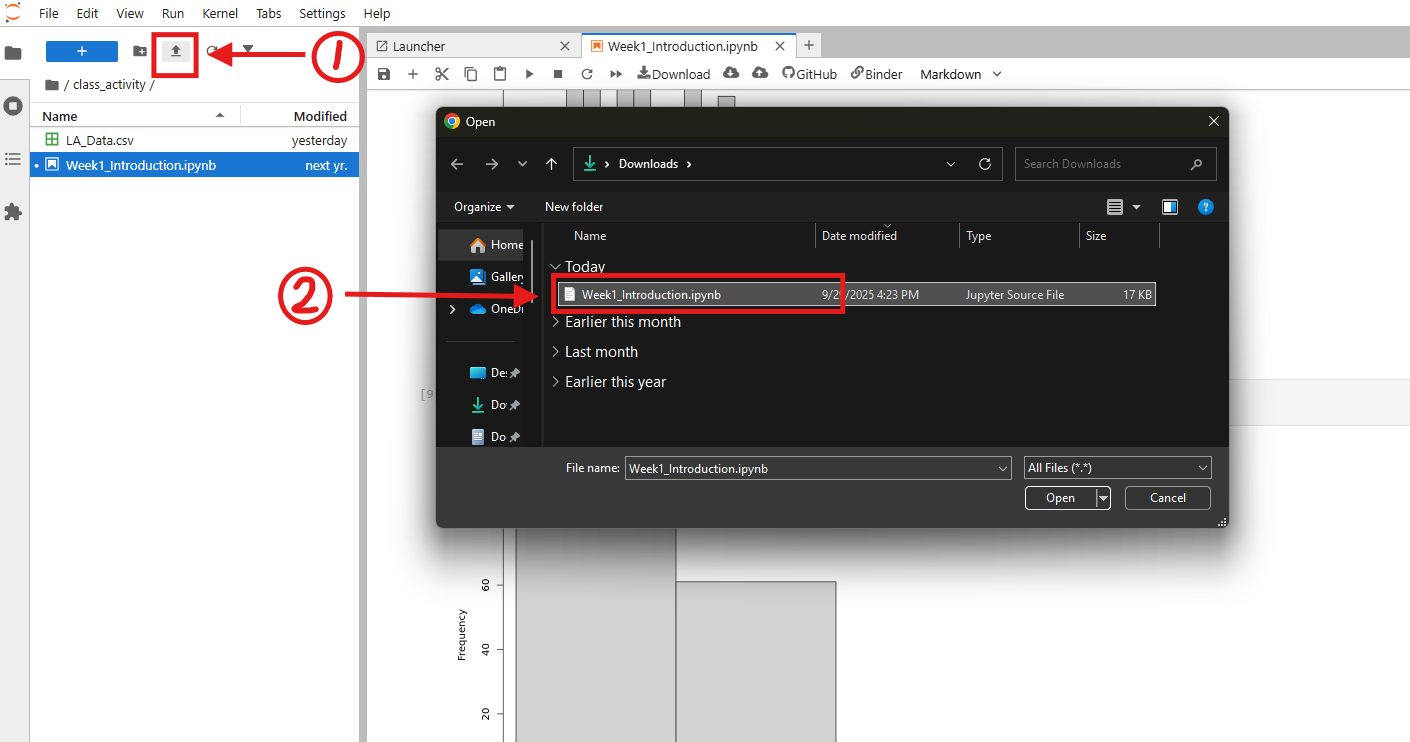
\includegraphics[width=0.8\textwidth]{../Image_12.png}\\
\textit{Use the Upload button to continue your work from where you left off}
\end{center}

\section{Need Help?}

\subsection{Contact Information}

\begin{infobox}
\textbf{Mohammadreza Narimani}\\
Email: mnarimani@ucdavis.edu\\
Department of Biological and Agricultural Engineering, UC Davis\\
Office Hours: Thursdays 10 AM - 12 PM (Zoom)
\end{infobox}

\subsection{Technical Issues}

\begin{itemize}
    \item \textbf{Binder won't load?} Try refreshing the page or clearing browser cache
    \item \textbf{Lost your work?} Always download files before closing Binder
    \item \textbf{Code not working?} Check for typos and make sure you've run all previous cells
\end{itemize}

\subsection{Learning Resources}

\begin{itemize}
    \item \textbf{R Documentation:} Use \texttt{?function\_name} in code cells for help
    \item \textbf{Course Materials:} All tutorials are in the \texttt{class\_activity} folder
    \item \textbf{Practice:} Try modifying the example code to learn more!
\end{itemize}

\section{What You'll Learn}

\begin{itemize}
    \item \textbf{R Programming Basics} - Variables, vectors, data frames
    \item \textbf{Data Visualization} - Histograms, plots, charts
    \item \textbf{Statistical Analysis} - Descriptive statistics, hypothesis testing
    \item \textbf{Agricultural Applications} - Real-world data analysis
    \item \textbf{Report Writing} - Professional statistical reports
\end{itemize}

\section{Tips for Success}

\subsection{Best Practices}

\begin{itemize}
    \item \textbf{Read instructions carefully} before starting each exercise
    \item \textbf{Run code cells in order} - later cells depend on earlier ones
    \item \textbf{Save frequently} - Download your work regularly
    \item \textbf{Experiment} - Try modifying code to see what happens
    \item \textbf{Ask questions} - Don't hesitate to reach out for help
\end{itemize}

\subsection{Keyboard Shortcuts}

\begin{itemize}
    \item \textbf{Shift + Enter} - Run current cell and move to next
    \item \textbf{Ctrl + Enter} - Run current cell and stay in place
    \item \textbf{A} - Insert cell above
    \item \textbf{B} - Insert cell below
    \item \textbf{DD} - Delete current cell
\end{itemize}

\section{Ready to Start?}

Visit the course website or click the Binder link to launch your first R programming session!

\begin{center}
\textbf{Happy coding!}
\end{center}

\vfill

\begin{center}
\textit{Last updated: October 2025 | PLS 120 - Applied Statistics in Agriculture | UC Davis}
\end{center}

\end{document}